\documentclass[a4paper]{article}

\usepackage[utf8]{inputenc}
\usepackage[T1]{fontenc}
\usepackage[francais]{babel}
\usepackage[top=2cm, bottom=2cm, left=2cm, right=2cm]{geometry}
\usepackage{graphicx}
\usepackage{float}
\usepackage{lmodern}
\usepackage{textcomp}
\usepackage{underscore}
\usepackage{longtable}
%\usepackage{hyperref}

\title{Analyse primaire}
\author{\bsc{Plateforme BioInformatique de Nantes}}

\begin{document}
\maketitle

\section*{Resumé Projet}
%Resume a écrire
Résumé non écrit

\section*{Description de l'engagement}
L'engagement comporte deux volets :
\begin{enumerate}
	\item Le premier est de fournir des données nettoyées et analysables. 
	\\ Cette partie comporte : 
	\begin{itemize}
		\item le contrôle qualité des échantillons, 
		\item la normalisation, 
		\item le filtrage des données 
		\item la visualisation des données par clustering hiérarchique. 
	\end{itemize}
	\item Le second est un guide pour l'interprétation biologique grâce à deux méthodes d'analyses :
	\begin{itemize}
		\item une analyse globale : recherche de cluster. 
		\item une analyse par gènes : analyse différentielle.
		\item annotation fonctionelle des clusters et des listes de gènes différentielles
	\end{itemize}
\end{enumerate}
 Les résultats de ces analyses seront sous la forme de listes de gènes associées à des fichiers d'annotations fonctionnelles. 
\\
L'ensemble de la démarche est décrite \bsc{Figure : }\ref{pipeline}.
\begin{figure}[H]
	\centering
		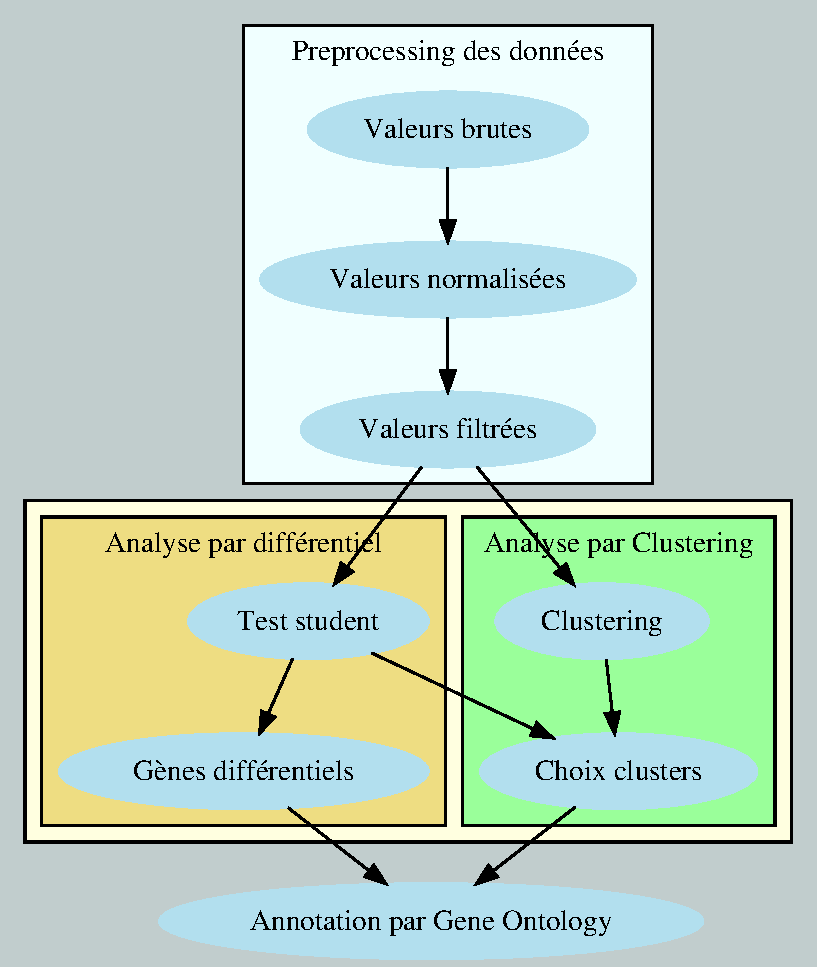
\includegraphics[scale=0.5]{workflow.pdf} 
		\caption{\label{pipeline} Etapes d'analyse primaire}
\end{figure}



\section*{Importation des données}

\input{importData}

%\subsection*{Matrice obtenue}
Note : sur la puce un gène peut être représenté par plusieurs sondes. Par abus de langage on peut utiliser le mot gène pour les sondes jusqu'à l'étape d'anotation.
\\
%Exemple matrice d'expression brute.(graph)
%\input{graphImport}


\section*{Normalisation}
Les données d'expression brutes sont normalisées selon la méthode de LOWESS 
En fonction d'un profil médian calculé à partir de la matrice de données d'expression. Pour chaque sonde on calcule son signal médian (la médiane).
\begin{itemize}
\item la normalisation LOWESS est une normalisation non linéaire. Elle fait une régréssion linéaire par fenêtre glissante.
\item cette normalisation est appliquée en fonction du \emph{profil médian} (médiane par ligne).
\end{itemize}
\input{graphNorm}

\section*{Contrôle qualité des échantillons}
\subsection*{Statistiques descriptives : boxplot}
\begin{itemize}
\item Le but des statistiques descriptives est de vérifier la distribution des données sur certaines valeurs d'expression pour chaque échantillon.
\item Elles sont réalisées avant et après la normalisation
\item Avant normalisation on s'attend à une différence d'intensité entre les deux dyes.
\item Après normalisation cet effet doit être corrigé : les courbes doivents être relativement planes
\end{itemize}


\textbf{Résultats :} \bsc{Figure}~\ref{statDes}.
\input{graphStatDesc}
\subsection*{Corrélation}
On calcule la corrélation de Pearson de chacun des échantillons par rapport à un Profil médian.
\par
Le profil médian est calculé à partir de la matrice de données d'expression. 
\par
Pour chaque sonde on calcule son signal médian (la médiane)
%\input{exempleProfilMedian}
De manière générale la corrélation varie entre -1(anti corrélé) et 1 (corrélé).
Si elle est égale à 0 il n'y a pas de corrélation.
\par
Nous considérons qu'une corrélation >= 0.8 est une bonne corrélation.
\\
\textbf{Résultats :} \bsc{Figure}~\ref{Correlation}.
\input{graphCorrelation}

\section*{Filtrage}
\begin{itemize}
\item Principe : éliminer les sondes proches du bruit de fond.
\item Plusieurs méthodes de filtrage sont possibles. Celle utilisée ici assume qu'environ la moitié des gènes ne sont pas exprimés dans le système étudié.
\item Il est possible de rajouter des sondes d'interêt pour l'analyse.
\input{filtrage}
\end{itemize}

\section*{Clustering hiérarchique}
\subsection*{But}
\begin{itemize}
\item Visualiser les données et determiner des problèmes dans la matrice d'expression.
\item Visualiser les signatures (regroupement des gènes).
\item Visualiser la classification des échantillons.
\item Déterminer des clusters d'expression différentielle.
\end{itemize}
La matrice est représentée par les sondes en lignes et les échantillons en colonne. Une couleur rouge montre une sur-expression de l'échantillon et une couleur verte une sous expression.
%\subsection*{Filtrage Clustering : signal median}
%\input{filtrageClustering}
\subsection*{Démarche par clustering (groupe de gène)}
\begin{itemize}
\item Pour chaque sonde un test statistique est effectué pour chaque question binaire et une Pvalue lui est attribué (voir plus loin pour l'explication de l'obtention de la pvalu et du test)
\item Les pvalue sont ordonnées selon le clustering. Des pics distinguent les clusters répondant à la question du test.
\item les pvalue sont reportées sur un graphique en appliquant la formule -log10(pvalue) afin de mieux visualiser les données
\item Afin de lisser la courbe nous calculons une \emph{moyenne mobile}. La moyenne des -log10(pvalue) est faite par pas de 200.
\end{itemize}
%\input{graphExempleCluster}
\section*{Résultats Clustering}
\subsection*{Questions Binaire}
\input{graphCluster}
%\input{clustBinaire}

\subsection*{Annotation Fonctionnelle}
Le principe est d'associer des annotations fonctionnelles aux clusters, en utilisant la base de données Gene Ontology (GO)\\
Pour ce faire nous utilisons le logiciel GOminer qui fournit pour chaque liste deux fichiers : 

\par

\IfFileExists{AnnotationCluster.tex}{\input{AnnotationCluster.tex}}

\begin{itemize}
	\item Un fichier \emph{*fdrse.txt} contenant les annotations GO associées à différentes informations
	\item Un fichier \emph{*gce.txt} contenant l'association des annotations et des gènes du clusters.
\end{itemize}
\begin{itemize}
\item En-tête du fichier \emph{*.fdrse.txt} :
\begin{description}
	\item[GoID : ] indentifiant de l'annotation dans la base GO 
	\item[Total : ] nombre de fois que l'annotation est retrouvée sur la matrice filtrée
	\item[Change : ] nombre de fois que l'annotation est retrouvée dans le cluster
	\item[Enrichissement : ] calcul de l'enrichissement de l'annotation
	\item[Pvalue : ] significativité de l'annotation
	\item[Term : ] description de l'annotation
\end{description}

\end{itemize}
\section*{Résultats gènes différentiels}
Pour chaque question binaire un test de student est effectué. On test si les moyennes des deux paramétres sont significativement différentes.
\\
Plus l'ont fait de test plus nous un risque d'obtenir des faux positif. Pour cela nous effectuons une correction des pvalue par la méthode de Benjamini-Hochberg.
\\
Le tableau ci-dessous représente le nombre de sondes significatives avec correction

\par

\input{genDiff.tex}

%\input{genDiffRaw.tex}

\par
\subsection*{10 meilleurs annotations fonctionnelles pour chaque fichier (up et down par question)}
\IfFileExists{annotGeneDiff.tex}{\input{annotGeneDiff.tex}}{Pas d'annotation fonctionnelles significatives}

%\section*{Niveau d'expression des génes d'interêts}
%\input{graphGene.tex}




%\section*{Utiliser les fichiers de résultats}
%\subsection*{Fichiers textes}
%Pour plus de facilités vérifier que votre système d'exploitation affiche bien les extension de fichiers.\\
%Tous les fichiers de résultats sont des fichiers textes tabulés ou des listes extension \emph{.txt}.\\
%Ces fichiers sont ouvrables avec Excel. Il existe plusieurs façon de procéder :
%\begin{itemize}
%\item Ouvrir Excel puis glisser le fichier dans la feuille vierge. 
%\item Executer Excel puis ouvrir un nouveau fichier.
%\item Clique droit sur le fichier et faire ouvrir avec et séléctionner Excel.
%\end{itemize}
%
%Important les décimales des nombres sont des points et non des virgules. 
%\\Il existe plusieurs façon de procéder.
%\begin{itemize}
%	\item Dans les options d'Excel changer les paramètres des décimales
%	\begin{itemize}
%		\item pour Excel 2003
%		\item pour Excel 2007
%	\end{itemize}
%	\item Remplacer les points par des virgules.
%\end{itemize}
%\subsection*{Fichiers clustering}
%Les fichiers de cluster possédent les extensions suivantes : atr, cdt gtr
%\begin{description}
%\item [atr et gtr : ] sont necessaires pour le tracé des arbres des échantillons et des gènes mais ils ne doivent pas être modifiés.
%\item [cdt : ] Le fichier lu par java treeview. On peut l'ouvrire avec Excel. Il contient la matrice clusterisé (les valeurs sont logé et centré médian sur les gènes).
%\end{description}

\section*{Outils d'analyse}
\subsection*{Utilisation de GOrilla}

\begin{description}
	\item [Étape 1 :]  choix de l'organisme parmis
		\begin{itemize}
			\item \emph{Homo sapiens}
			\item \emph{Mus musculus}
			\item \emph{Rattus norvegicus}
			\item \emph{Arabidopsis thaliana}
			\item \emph{Saccharomyces cerevisae}
			\item \emph{Caenorhabditis elegans}
			\item \emph{Drosophila melanogaster}
			\item \emph{Danio reiro}
		\end{itemize}
	\item [Étape 2 :] Choisir le mode \emph{Two unranked lists of genes (target and background lists)}
	\item [Étape 3 :] Fichiers d'entrée  
		\begin{description}
			\item [Target set : ] Liste de gènes, typiquement la liste d'un cluster.
			\item [Background set : ] Liste de toutes les gènes de la puce.
		\end{description}
	\item [Étape 4 Ontology : ] Sélectionner \emph{All}
	\item [Advanced parameters : ]  Cocher 
		\begin{itemize}
			\item \emph{Output results in Microsoft Exel format}
			\item \emph{Show also in REVIGO}
		\end{itemize}
	\item[Executer GOrilla] \emph{Search Enriched GO terms}
\end{description}


\section*{Info Session R}
\input{info}
\end{document}

